\chapter[Análisis de los algoritmos]{\label{identificadorReferenciaCruzada}
Análisis de los algoritmos}

En este capítulo nos centraremos en el análisis de los tres algoritmos explicados en el anterior, para ello haremos un anáisis a posteriori en un ordenador con las características mostradas en la tabla \ref{Tabla4}:

\begin{table}[h!]
\begin{center}
	\resizebox{5cm}{!}{ 
	\begin{tabular}{| l | r |}
		\hline 
			Procesador & Intel Core i7-2600 3.4GHz \\
				\hline 
			Memoria RAM & 32Gb DDR3 \\
		\hline
			Disco Duro &  Samsung SSD 850 EVO 120Gb\\
		\hline
			Sistema operativo.& Windows 7 profesional 64-bits\\
		\hline
			Tarjeta gráfica & Nvidia GeForce GT-430\\
		\hline
			
	\end{tabular}
	}
\end{center}
\caption{Características del ordenador} \label{Tabla4}
\end{table}

\section{Tiempos de ejecución:}

Para los algoritmos hemos realizado distintas ejecuciones con valores de la forma:

\begin{itemize}
	\item 10x10
	\item 20x20
	\item 30x30
	\item 40x40
	\item 50x50
	\item 60x60
	\item 70x70
	\item 80x80
	\item 90x90
	\item 100x100
\end{itemize}

Si nos damos cuenta, estamos realizando divisiones cada vez mayores para comprobar como aumenta el tiempo en cada algoritmo. Tras las distintas ejecuciones nos sale lo mostrado en \ref{Tabla5}

\begin{table}[h!]
\begin{center}
	\resizebox{15cm}{!}{ 
	\begin{tabular}{| c | c | c | c | c | c | c | c | c | c | c |}
		\hline 
			Algoritmo & 10x10 & 20x20 & 30x30 & 40x40 & 50x50 & 60x60 & 70x70 & 80x80 & 90x90 & 100x100 \\
				\hline 
			Primer algoritmo &  2.05	& 3.32	& 4.34	& 4.65	& 5.06	& 7.50	& 11.65	& 16.49	& 27.31	& 44.67\\
		\hline
			Segundo algoritmo & 9.47	& 24.70	& 67.09	& 155.33	& 278.37	& 446,81	& 1144.14	& 1240.22	& 1500.64	& 1924.82\\
		\hline
			Tercer algoritmo & 1.09	& 1.23	& 1.34	& 5.01	& 10.14	& 13.9	& 28.21	& 30.64	& 36.88	& 64.91\\
		\hline
	\end{tabular}
	}
\end{center}
\caption{Tiempo de ejecución (s) de los algoritmos para los distintas divisiones.} \label{Tabla5}
\end{table}


Como podemos ver, el tiempo en el segundo algoritmo es mayor, también se ha explicado anteriormente que es el más complejo, por otra parte, si representamos esos datos en gráficas de R nos daría lo mostrado en la figura \ref{Figura10}.

\begin{figure}[h!]

	\centering
	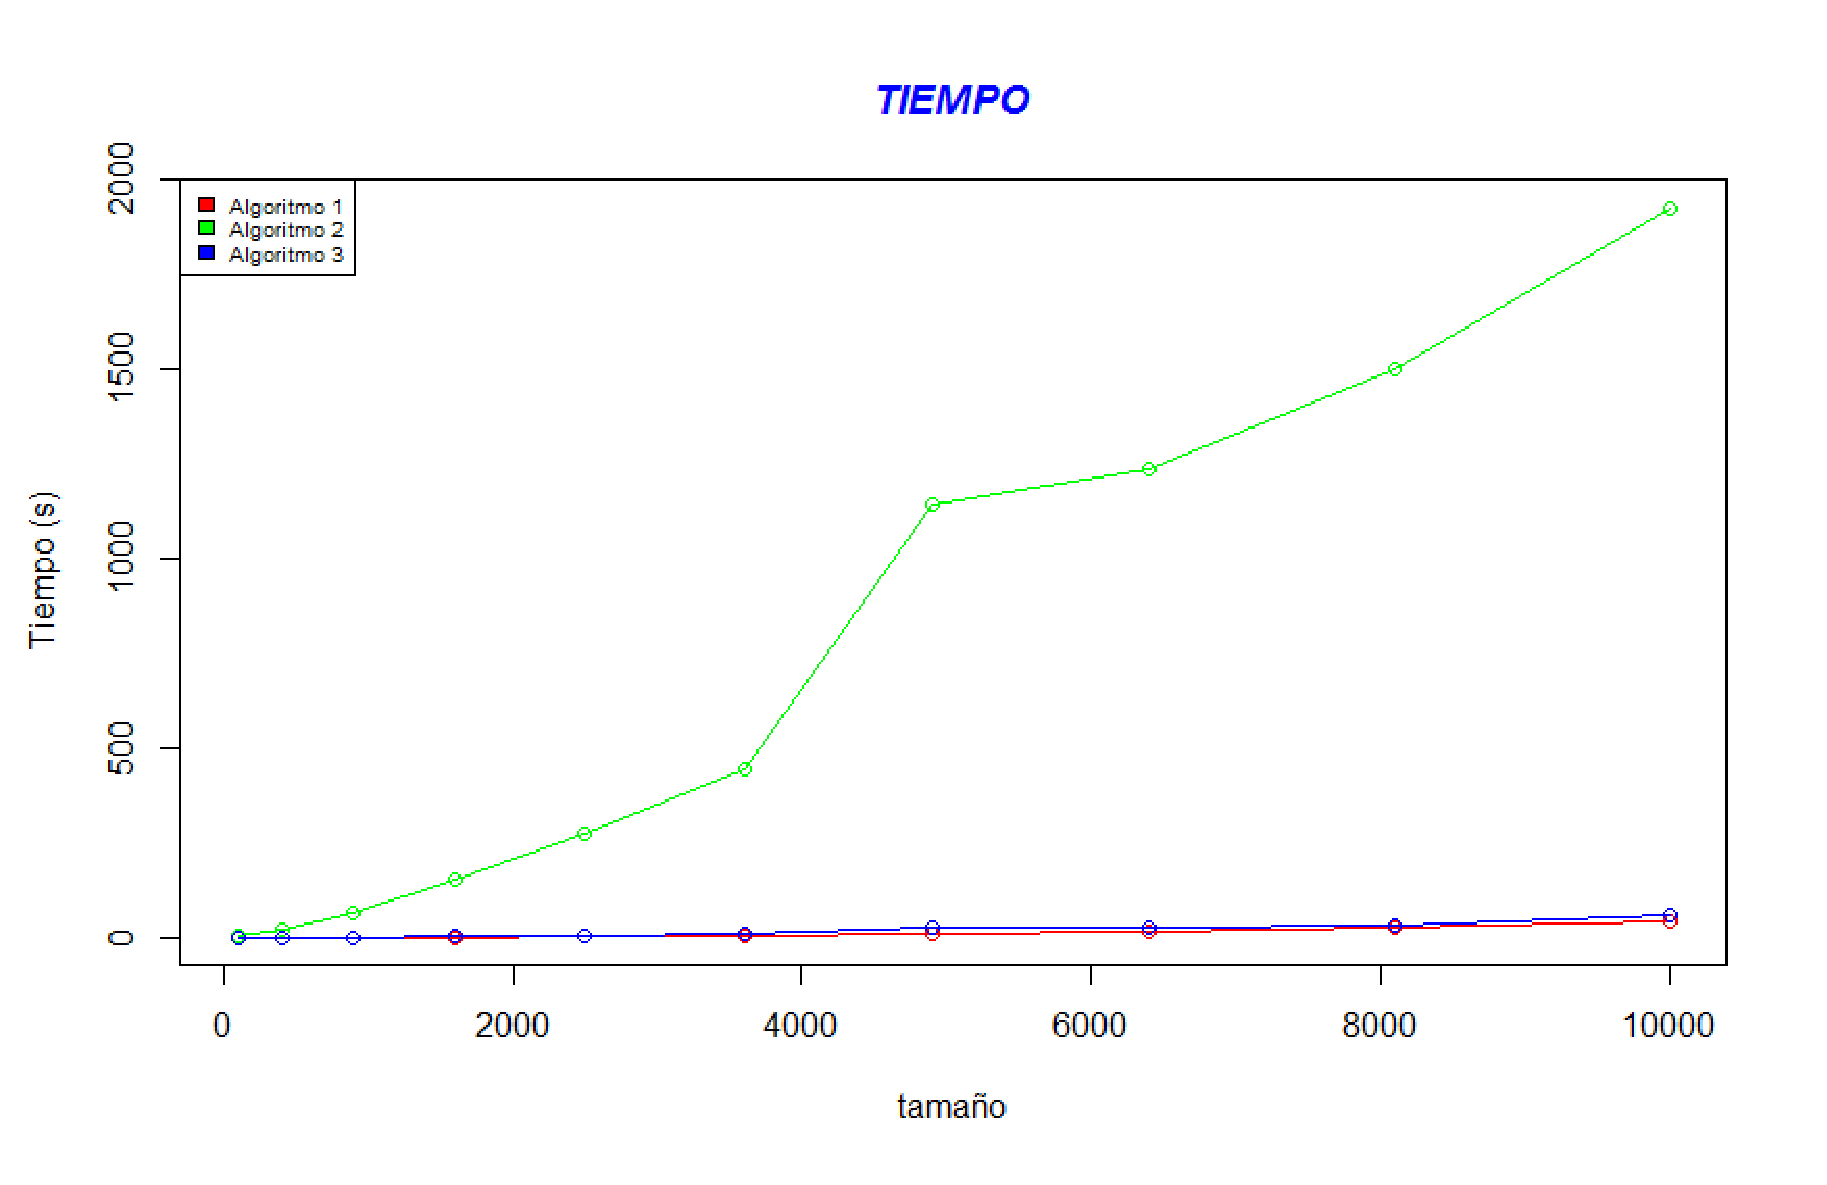
\includegraphics[width=8cm]{./eps/tiempo.eps}
	\caption{Representación gráfica en R de los tiempos de ejecución.}
	\label{Figura10}

\end{figure}

Con los datos representados, es trivial ver que los algoritmos, son de la forma \textbf{O$(n)$}. Para mostrarlo mejor, en la figura \ref{Figura11} podemos ver las gráficas de los algoritmos además del gráfico de O$(n)$ y de O$(n^2)$.

\begin{figure}[h!]

	\centering
	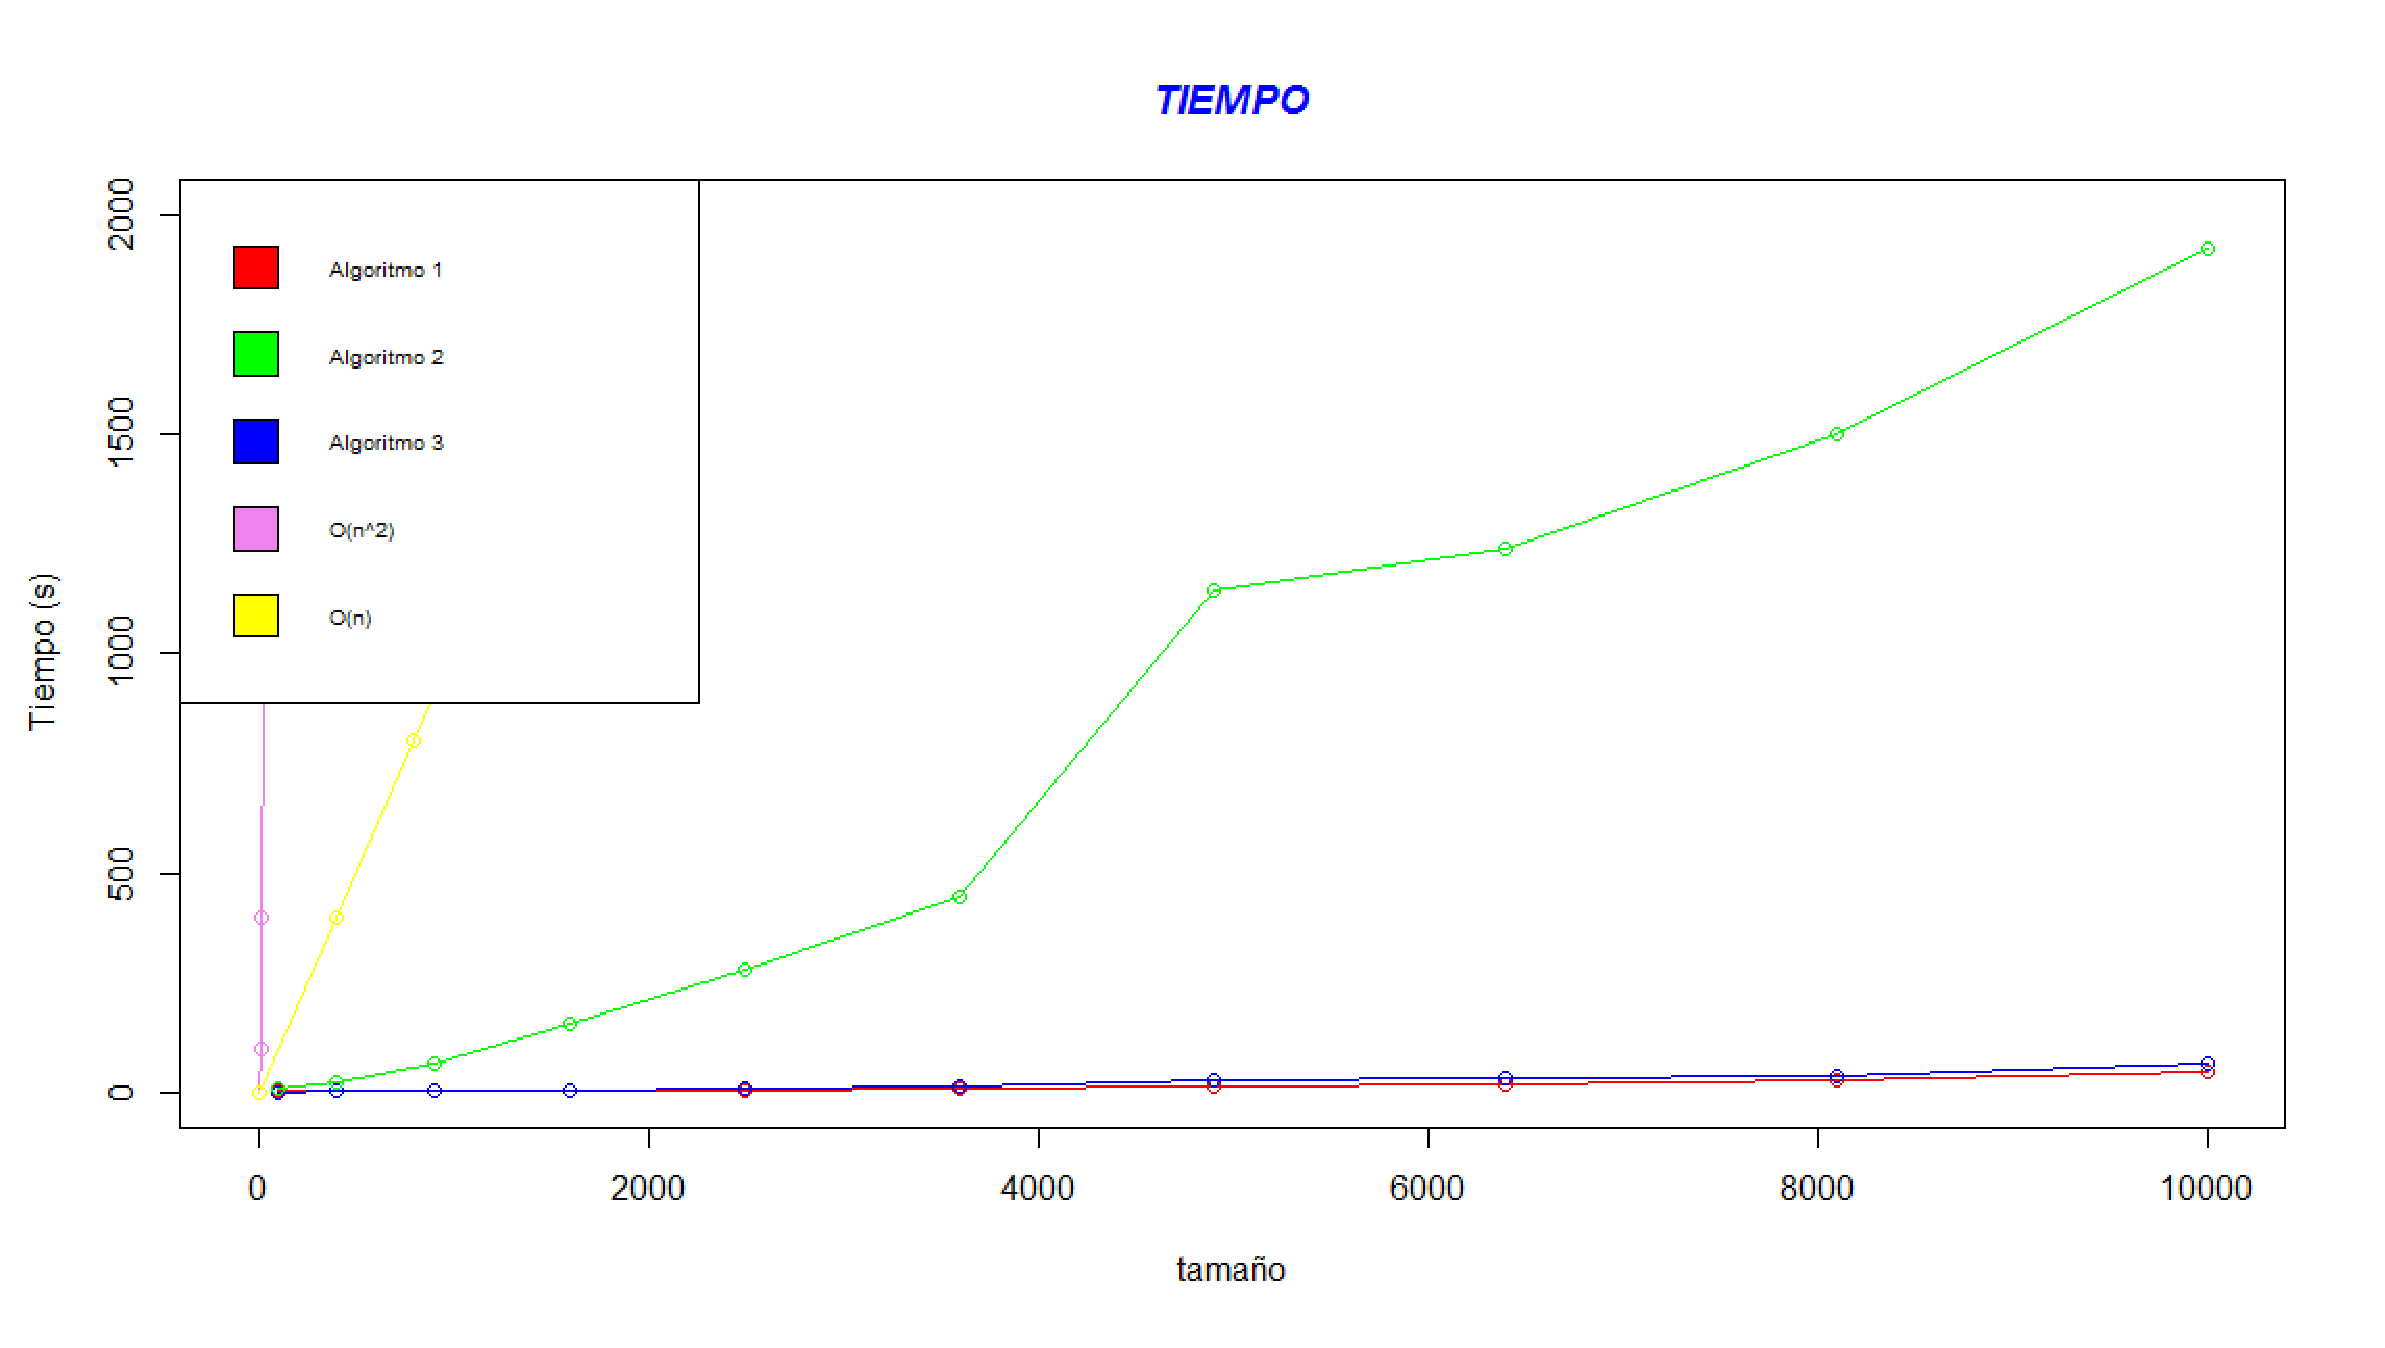
\includegraphics[width=8cm]{./eps/tiempofinal.eps}
	\caption{Comparación de tiempos con O$(n)$ y O$(n^2)$,realizada en R.}
	\label{Figura11}

\end{figure}

\section{Memoria:}

Para el estudio de la memoria utilizada por cada algoritmo hemos realizado la misma cantidad de ejecuciones con el mismo tamaño, dando los resultados indicados en \ref{Tabla6}


\begin{table}[h!]
\begin{center}
	\resizebox{15cm}{!}{ 
	\begin{tabular}{| c | c | c | c | c | c | c | c | c | c | c |}
		\hline 
			Algoritmo & 10x10 & 20x20 & 30x30 & 40x40 & 50x50 & 60x60 & 70x70 & 80x80 & 90x90 & 100x100 \\
				\hline 
			Primer algoritmo &  1.81 & 	1.85 &	1.87	& 1.95	& 2.11	& 2.23	& 2.38	& 2.53	& 2.64	& 2.82\\
		\hline
			Segundo algoritmo & 2.27 &	3.81 &	5.12	& 7.77 &	10.9 &	14.1 &	19.4 &	24.1 &	29.6	& 31.8\\
		\hline
			Tercer algoritmo & 0.5	& 0.68	& 0.80	& 1.01	& 1.25	& 1.50	& 1.93	& 2.12	& 2.28	& 2.50\\
		\hline
	\end{tabular}
	}
\end{center}
\caption{Memoria RAM (Gb) utilizada en cada ejecución de los distintos algoritmos.} \label{Tabla6}
\end{table}


Por otro lado hemos analizado la memoria que utiliza cada uno de los algoritmos en las distintas ejecuciones para que el usuario que vaya a trabajar con la biblioteca, pueda elegir que algoritmo le conviene más. En la figura \ref{Figura12} podemos ver la cantidad de memoria RAM utilizada por cada algoritmo.

\begin{figure}[h!]

	\centering
	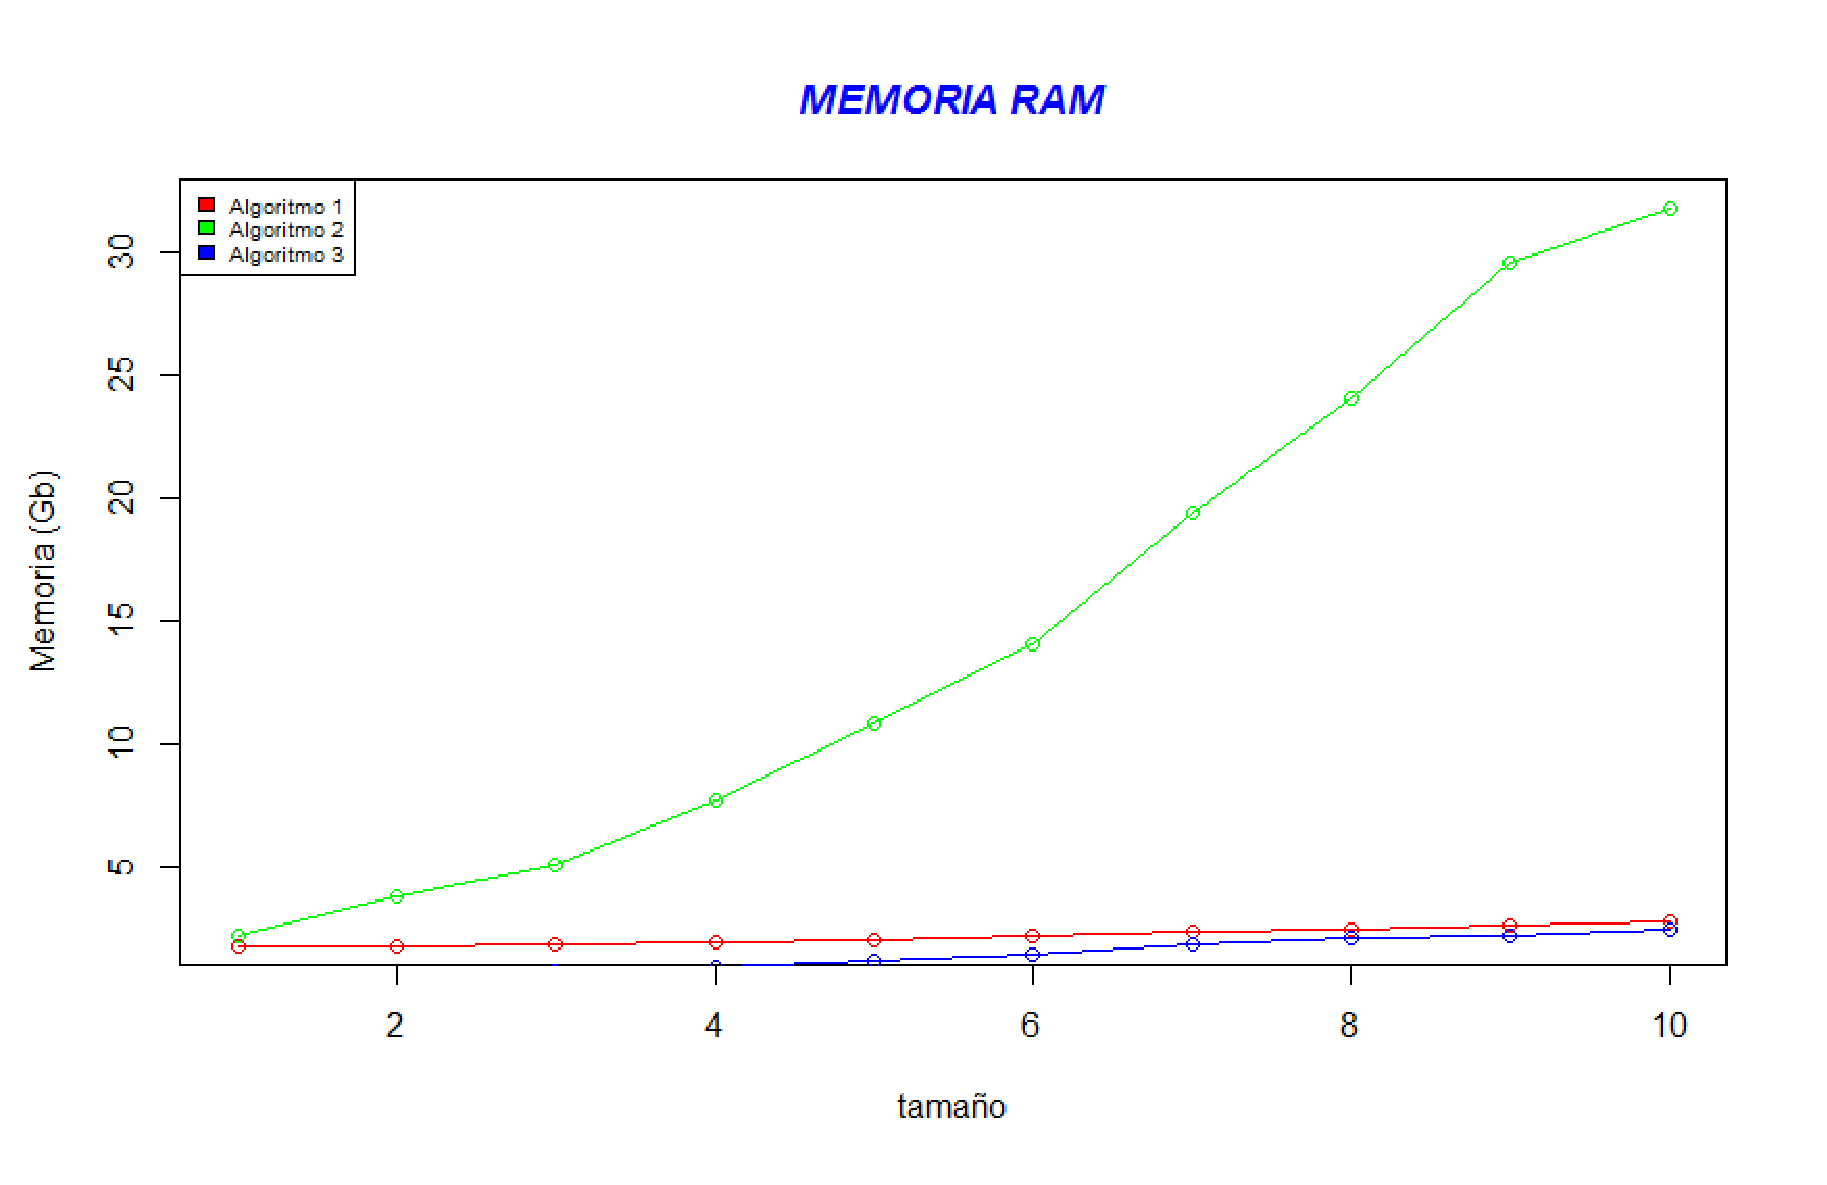
\includegraphics[width=8cm]{./eps/memoria.eps}
	\caption{Memoria RAM (Gb) utilizada por los distintos algoritmos según ejecución, realizada en R.}
	\label{Figura12}

\end{figure}

Como podemos ver, la cantidad de memoria utilizada por el segundo algoritmo, es mucho mayor, deja al ordenador casi sin memoria en la última ejecución, mientras que el primero y el tercero usan una cantidad de memoria bastante razonable y que se puede usar en cualquier juego.


\section{Conclusiones:}

Las conclusiones obtenidas de los últimos puntos son:

Los algoritmos primero y tercero pueden ser utilizados en cualquier juego, realizando tamaños de ciudades tan grandes como se deseen, mientras que el segundo algoritmo, sólo se puede utilizar en tamaños pequeños, si deseamos usarlo en cualquier juego, en el caso de querer ciudades grandes y con tanto detalle como este algoritmo nos las muestra, el juego tendría que tener calidad, y los requisitos mínimos para el funcionamiento de este serían bastante mayores.

\newpage






